%\begin{figure}[htb]
\begin{teaserfigure}
  \centering
  \subfloat[scene representation]{
    \label{fig:teaser:scene}
    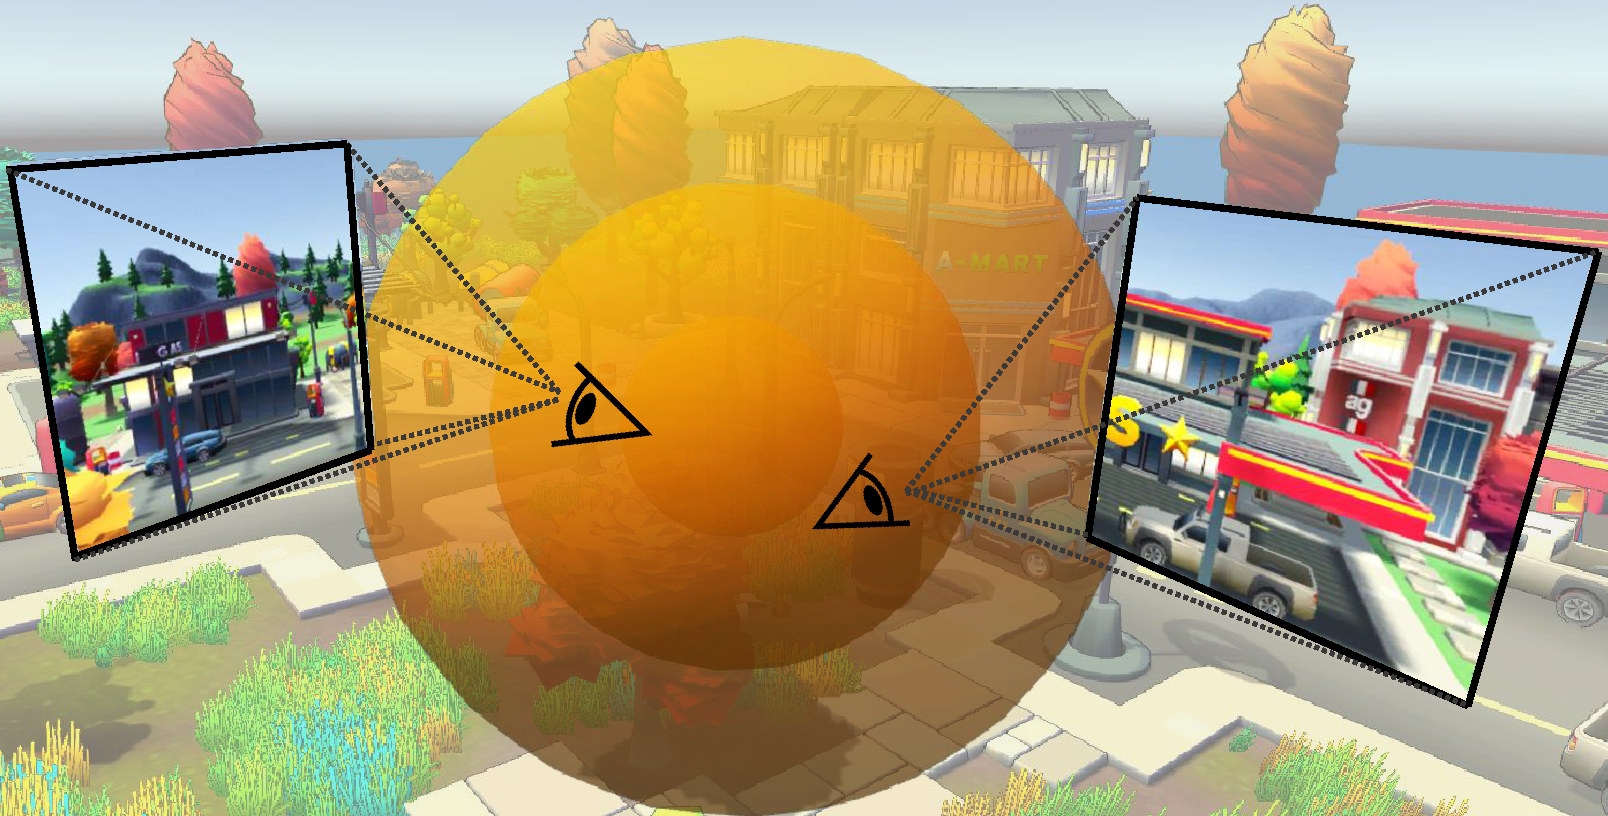
\includegraphics[width=0.45\linewidth]{TOG/figs/scene.pdf}
  }%subfloat
  \subfloat[latency]{
    \label{fig:teaser:latency}
    \includegraphics[width=0.25\linewidth]{example-image-a}
    % nerf: 108s/per infer
  }%subfloat
  \subfloat[quality]{
    \label{fig:teaser:quality}
    \includegraphics[width=0.25\linewidth]{example-image-a}
  }%subfloat
 \Caption{Illustration of our system.}
 {%
\subref{fig:teaser:scene} shows visualizes our active-viewing tailored scene representation.
Comparing with \protect\cite{mildenhall2020nerf}, \subref{fig:teaser:latency} shows our benefits of reduced latency.
As a zoom-in, \subref{fig:teaser:quality} compares our foveal quality preservation.
\qisun{Cross out half-half in  \subref{fig:teaser:hmd}. TODO for myself: I should make the background scene semi-transparent. Will do so soon.}
 }
 \label{fig:teaser}
%\end{figure}
\end{teaserfigure}
